\documentclass[12pt, letterpaper]{article}
\usepackage[utf8]{inputenc}
 \usepackage[letterpaper, margin=1in]{geometry}
 \usepackage{amssymb}
\usepackage{amsmath}
 \usepackage{enumitem}
\usepackage {listings}
\usepackage{pgfplots}
\usepgfplotslibrary{external}
\usepackage{graphicx}

\title{CS461 PA 3: \\cexpr - calculator for C integer expressions }
\author{Ksenia Burova}
\date{October 21st, 2017}

\begin{document}
 
\maketitle

\noindent {\bf Abstract:}\\
In this programming assignment, the goal was to write a program using yacc and lex that implements a calculator of C integer expressions.  
The calculator would process expressions until  EOF or invalid syntax. Each calculation would be terminated by a semicolon and tokens may be separated by whitespace. After each calculation, the calculator would print its result, no matter if it was an assignment or not. Tokens include integer
numbers and 26 predefined integer variables (a-z). The table with C operators to implement was given where operators were listed in order of decreasing precedence. \\
	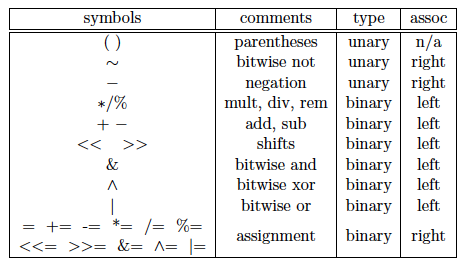
\includegraphics[scale=0.6]{1.png}

\noindent {\bf Programming approach:}\\
I've started this lab by looking at the provided {\bf .y} and {\bf .l} files. There was a little bit of syntax given which was helpful. I was adding rules to  {\bf .y} and  regular expressions to {\bf .l} files one at the time since this programming environment was new to me and I tried to avoid bugs. I've started with simple rules like addition and multiplication, and made them to work. Then added an assignment, made it to work as well. And so on. I had to google a few things, when I had unknown bugs, or wasn't sure about yacc syntax.

\begin{itemize}
	\item {\bf Design} \\
	I tried to keep design as it was given. I also tried to indent everything to make it readable. I avoided comment since it is obvious in all statement what's going on.
	\item {\bf Testing:} \\
	For testing I wrote some C expressions in a separate file. And wrote a shell script that runs that file with my and given .cexpr, and compares results. Here are tests I ran:
	\begin{verbatim}
		a = 55-3;
b = c = a-42;
a+b*c;
dump;
clear;
c = 6;
a = b;
a = 10000;
b = 100000;
a*b;
a*b*10;
c/d;
d/c;
a += b += c -= 7*3;
d = (17+5)*3 - 8*(1+7)/2;
g = -a;
h = - -a;
i = ~b;
dump;
z = w = a * ( 17/4%2 + 3%2 );
25 >> 12;
12 << 25;
12 << -1;
1230 << 33;
h = d <<= 8;
h >>= 4;
c %= 2;
k = 324;
dump;
m = 2423;
k |= m;
k &= 162;
m ^= 26;
z /= 0;
dump;
z /= 12;
o = 12 | 3 | 4;
p = 12 | 4 ^ 5;
q = (12 | 4) ^ 5;
(12 | 4) ^ 5 & 3;
dump;
(12 | 4 ^ 5) & 3;
x = 4^4;
l ^= q ^ m;
f = 10000000;
f * 10000000000;
f = -111111111111111111;
((5 & 6) << 3 * ~( (-1 - 2) ^ ( 25 >> 2) )) & 1000 / 34 / 2 * (6 - 8);
m = ~~56;
clear;
	\end{verbatim}
	\item {\bf Debugging:} \\
	For debugging I used regular {\it printf} statements inside of my rules and functions. I also tried to compare results against output from given executable along the way.
	 \item {\bf Issues:} \\
	There were multiple issues with assignment. First, lack of yacc syntax knowledge. But that didn't take a long time to learn. Then, knowing what output to expect on overflow. For example, left shift overflow must happen on left shift by negative number, but given program gives zero. I return {\it overflow} since it's what should be. Also testing against other overflows was sort of iffy. Wasn't sure how to define rules at first. Handling read-in of too large number made me stuck for a second as well. Lastly, there were not that many test cases given by instructor, so I'm not sure if I hit all the possible test cases myself. I hope I did. 
\end{itemize}

\end{document} 